\documentclass[final]{article}

% if you need to pass options to natbib, use, e.g.:
% \PassOptionsToPackage{numbers, compress}{natbib}
% before loading nips_2017
%
% to avoid loading the natbib package, add option nonatbib:
% \usepackage[nonatbib]{nips_2017}

\usepackage{nips_2017}

% to compile a camera-ready version, add the [final] option, e.g.:
% \usepackage[final]{nips_2017}

\usepackage[utf8]{inputenc} % allow utf-8 input
\usepackage[T1]{fontenc}    % use 8-bit T1 fonts
\usepackage{hyperref}       % hyperlinks
\usepackage{url}            % simple URL typesetting
\usepackage{booktabs}       % professional-quality tables
\usepackage{amsfonts}       % blackboard math symbols
\usepackage{nicefrac}       % compact symbols for 1/2, etc.
\usepackage{graphicx}
\usepackage{microtype}      % microtypography

\title{Deep Learning for Music Generation}

% The \author macro works with any number of authors. There are two
% commands used to separate the names and addresses of multiple
% authors: \And and \AND.
%
% Using \And between authors leaves it to LaTeX to determine where to
% break the lines. Using \AND forces a line break at that point. So,
% if LaTeX puts 3 of 4 authors names on the first line, and the last
% on the second line, try using \AND instead of \And before the third
% author name.

\author{
   Peter  Schaldenbrand\\
  Human-Computer Interaction Institute \\
   Carnegie Mellon University \\
     Pittsburgh, PA 15213 \\
   \texttt{pschalde@andrew.cmu.edu} \\
     \And
   Yizhou He \\
  McWilliams Center for Cosmology\\
  Dept. of Physics \\
  Carnegie Mellon University\\
  Pittsburgh, PA 15213 \\
  \texttt{yhe2@andrew.cmu.edu} \\
    %% examples of more authors
  \And
   Husni Almoubayyed\\
  McWilliams Center for Cosmology\\
  Dept. of Physics \\
  Carnegie Mellon University\\
  Pittsburgh, PA 15213 \\
  \texttt{halmouba@andrew.cmu.edu} \\}

\begin{document}
% \nipsfinalcopy is no longer used

\maketitle

\section{Introduction}

\paragraph{}Music is not currently a common area of interest in the machine learning community.  While much attention is given to text, speech, and images, music remains a domain that lacks focus from many researchers.  Among the many reasons for this neglect is the difficulty of learning from musical data.  For instance, a piano has 88 keys which means that there can be up to $2^{88}$ different combinations of keys that an artist could strike.  Across most representations, the dimensionality of musical data can be massive.  Music, when it is stored in raw form such as .wav or .mp3 files, is often sampled at 48 kilohertz and it is common that each sample is 16 bits in size.  Given this rate at which music is stored, standard song lengths are explosive in data size when looking at raw music.  MIDI is a communication protocol that specifies the pitch of a musical note, the velocity at which it is played, the instrument playing it, the tempo of the music, and a few other details.  This makes a much more compact representation of music than raw data.  But even so, the dimensionality of MIDI data can be very large with the possible number of combinations of notes and their lengths.
\paragraph{}Given the large dimensionality and complexity of music data, we found it necessary to use deep learning algorithms to model the intricacies of music and its structure.  We fortunately found a large dataset of MIDI files for our complex learning algorithms to be able to learn commonalities across all music.  Recurrent Neural Networks [11] are designed for time series data and can produce streams of data by predicting the next sound given a history of sounds in a song unlike Generative Adversarial Networks [9] which can only produce a fixed output of generated music.  Long Short-Term Memory [12] units can make an RNN more powerful by using an even longer and finer tuned history of the song to generate new segments of the song.  In this paper, we will use an LSTM network to generate music since one of our goals is to produce a continuous stream of music.
\paragraph{}The largest music generation project is Magenta by Google [1].  Magenta uses LSTMs to generate music, and provides programs to extract melodies from MIDI files.  Magenta uses an assumption that the music it is trained on and generating is from one source and instrument. We will try to use Magenta as a starting point and attempt to build a system with less assumptions about music and generate music that sounds more like a human produced it.  We will build our model using a high-level neural networks API, \texttt{Keras} [14].  Although \texttt{Keras} is a high-level tool, it provides the ability to make fine grain changes to the machine learning model.
\paragraph{}Our choice to use MIDI files as the type of our training data was not random.  Some of the latest research in generating music is using raw files to train very complex models.  WaveNet [2] use a stacked convolutional layers without max pooling to create a very complex model that can generate audio.  WaveNet was able to produce believably piano-created music, and given the complexity and size of raw music this is very impressive.  However, the particular music that the model generated was not very interesting.  Raw music data seems to be too complex for current machine learning algorithms to learn the nuances and beauty of the music.  On the other hand is MIDI data which provides a much simpler representation of music, but prior works such as [7], [5] and [6] still use many assumptions about music in their models such as tempo, genre, key, and rhythm.  We would like to meet in the middle of these two ends of the musical machine learning complexity spectrum and produce music using a model with very few assumptions about music.

\section{Related Work}
\paragraph{}Early work in music generation algorithms predominantly puts large assumptions into the models.  To account for musics large dimensionality and lack of large, high quality datasets, researchers needed to fine tune their systems so they could learn the structure of melodies and rhythms easier.  In [5], they take several commonalities of music and use them to their advantage to train their model.  They only use blues music, the chords did not vary per song, no rests were predicted, and only quarter, half, and whole notes. Another paper that constrained its model to only be trained on one genre of data was [6].  Their model was trained on a data set consisting only of MIDI files that were performances of Johann Sebastian Bach\rq s music.  They state that two issues with this model were that the model did not separate melody from accompaniment, and that it did not predict when notes ended, only when they began.
\paragraph{}There were two evaluations scores used in [6]; accuracy and F1.  They point out that these evaluation functions do not necessarily correspond to human perception of music similarity.  This inspired us to write our own loss function that might be able to capture a humans\rq perception of correctness of predicted pitch or note.  Another paper that confirmed the usefulness of a unique loss function for the nature of musical data tried to predict melodies and used rules to determine how successful the generated melodies were.  [13] used evolutionary algorithms to find a neural network that maximized the chance of generating good melodies.  To compare melodies, they used composition rules on tonality and rhythm including rules inferred from Bela Bartok\rq s music.  [13] views music as a language and tries to represent specific melodies.
\paragraph{}While most of music generation algorithms focus on learning a prediction function directly, one of the prior works that we came across makes an attempt to model the distribution of data.  In [3] Restricted Boltzmann Machines (RBM) were used to model the distribution of notes at each timestamp in music.  On top of the RBM an RNN is used to generate actual music.  One particular shortcoming of this method was that the generated music was not able to capture longer-term musical structure.
\paragraph{}The most similar previous work that we found to ours is [4], who use a two layer LSTM to generate music.  Their goals were to find a meaningful representation of music as a vector and to use a neural network to express the notions of harmony and melody.  They also use MIDI files, however they normalized the ticks per beat in their data.  The LSTM used cross-entropy loss and was only trained on music composed by Bach.  They found that their model could not learn the "on-off" structure of MIDI files and therefore generated music with many rests or unappealing long notes.

\section{Method}

\paragraph{}Each note in a piece of music has a pitch, velocity, duration and etc, and in any composed music, there exist long term pattern in these features.  LSTM, where long short-term refers to memorizing short term for a long time, and is suitable for recognizing and capturing time-series data, and thus well-suited for music.  A more recent development in deep learning than an LSTM is GAN [9].  GANs have been used to generate music, but there have been some shortfalls, such as its inability to produce continuous streams of music and fall short in producing believably human music [10]. [8] on the other hand, we decided to go with LSTMs since LSTMs use a long amount of the history of the data in a song to predict the next data point.
\paragraph{}Our feature vector is composed of four variables: musical note, velocity, change in time from previous vector, and duration of note. We have plans to experiment with additional features such as tempo, key, and key signature; however for the time being, we are only using the note to make predictions.
\paragraph{}We start with a simple architecture similar to that used in [4]. Our current LSTM neural net contains 3 layers: the first layer contains 13 LSTM neurons, second layer contains 13 LSTM neurons and last layer provides the output via a softmax function that returns the probabilities of the different notes, the highest probability classifies the output note. We also apply a dropout coefficient 0.3 to prevent it from overfitting. A sequence with a length of T time steps $X_i, X_{i+1}, \dots , X_{i+T}$ of input vectors are fed into the LSTM, which then predicts the $X_{i+T+1}$th note. We use the categorical cross-entropy loss function. When doing the prediction we pick the first T time steps of music feature vectors of a song $X_1, X_2, \dots ,X_T$  as input sequence and get the first prediction $X_{T+1}$ from our trained LSTM network, use $X_2, X_3, \dots ,X_{T+1}$ as the new input sequence to generate new prediction, repeating this procedure leads us to our generated song.   
\paragraph{}This simple loss function has provided us with promising output but we plan to implement a custom algorithm to help our model generate better music.  Currently, the loss on the prediction of a note grows with distance from the true note.  However with music, if a predicted note is in harmony with the true note, this should produce a smaller penalty than predicting a note that is completely wrong.

\section{Dataset}
We decided to compile our own dataset for use in this project. The data is midi files collected online from sources under licenses allowing free usage for research purposes. A midi data file comprise of an array of messages, each consisting of the channel number (0 to 15); the note value; the velocity, representing how hard a note was hit; whether the message indicates that the note is being turned on or off; and a time-delta, representing the amount of time (in units of ticks) since the last message on the same channel. Midi files also include other metadata such as the tempo and time signature. As we are collecting the data, it is being pushed on to github, at \texttt{https://github.com/hsnee/DeepLearning4Music/tree/master/data}, mostly organized by genre. We use the python library \texttt{mido} to read in the midi files [15]

\section{Preliminary Results}
\paragraph{}At this point, we have generated music, using only an array of the note values from midi files. Figure 1 shows a transcription of the music that the LSTM composed, starting off from 13 previous data points that were extracted from one of the midi files. The results are in the correct format and are a preliminary output of what to expect from the final music generated by the LSTM, after several improvements explained in the next section. The training accuracy that we achieved on a small subset of the data with categorical cross-entropy loss and 200 epochs is 68.3\%. 

\begin{figure}[htbp]
\begin{center}
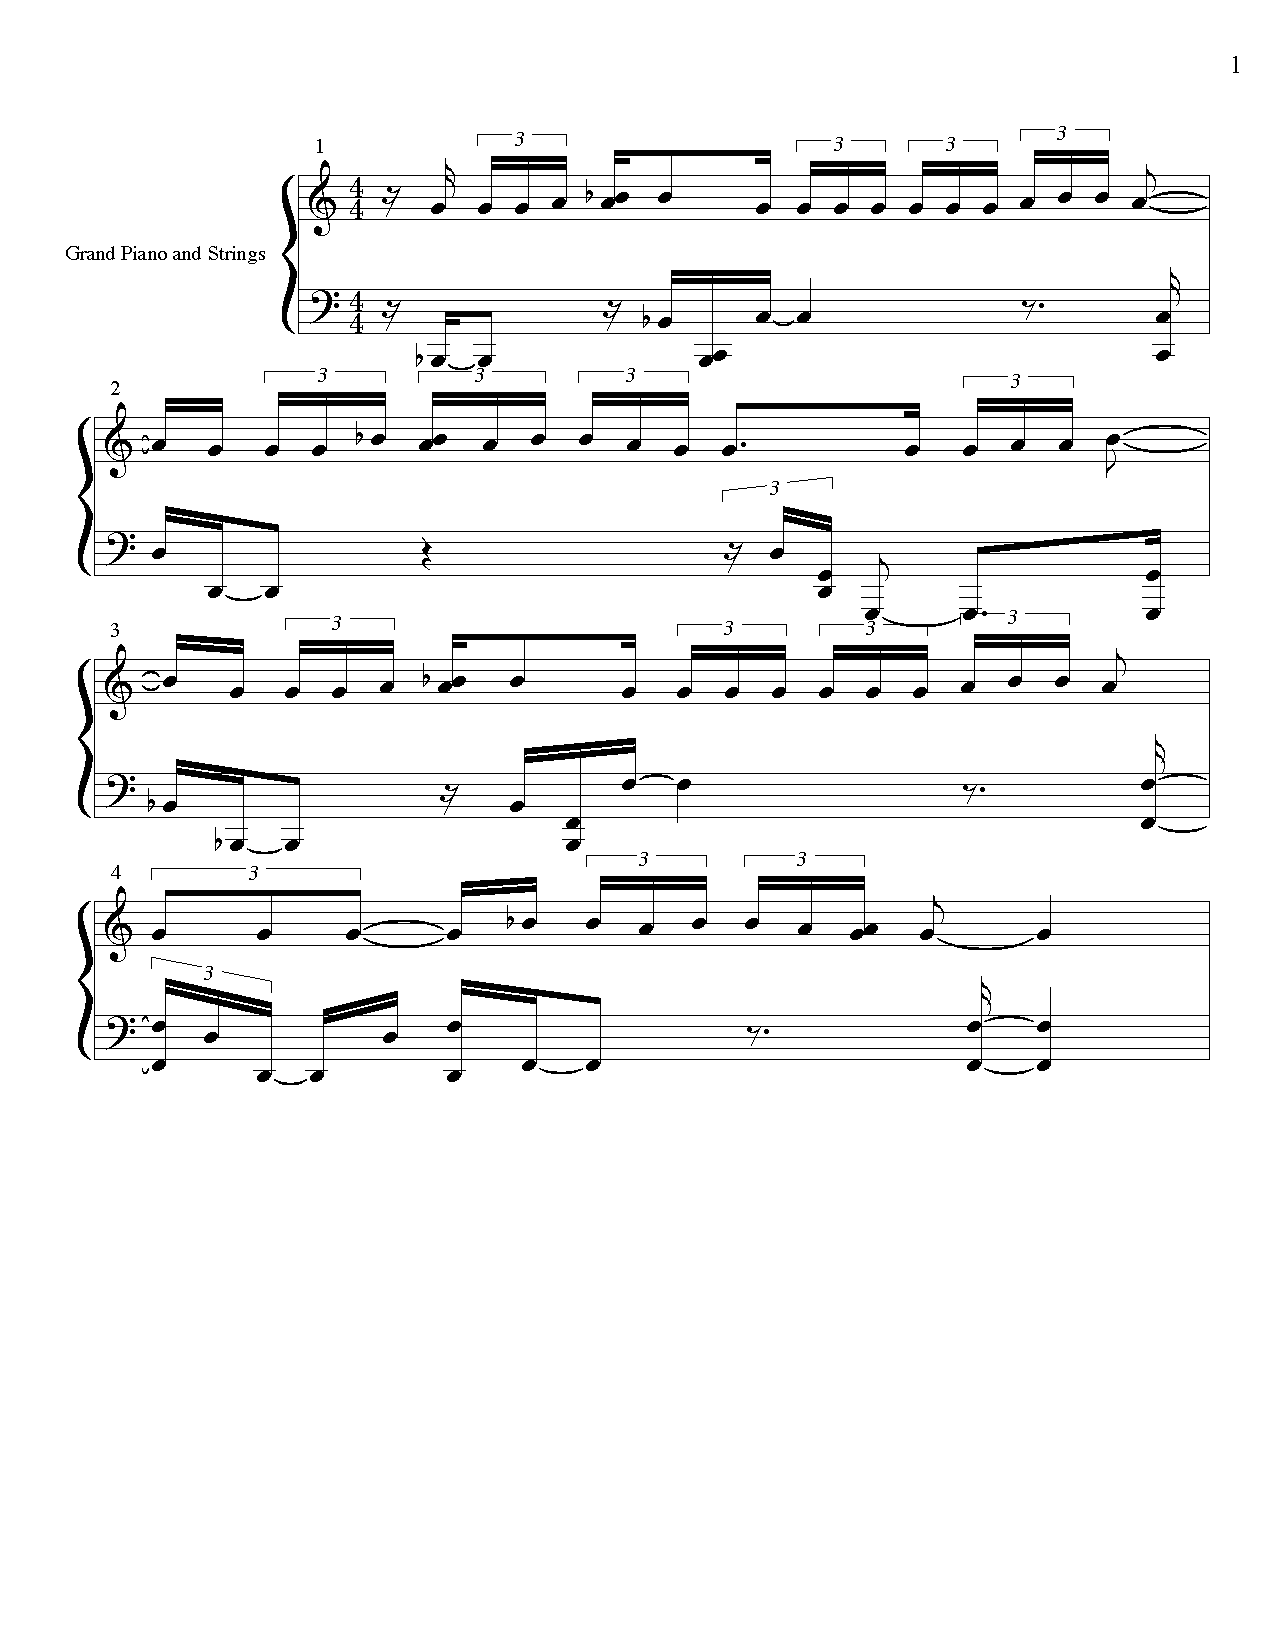
\includegraphics[width=\textwidth]{1stsong.png}
\caption{Prediction result from the }
\label{default}
\end{center}
\end{figure}


\section{Timeline and Future Work}

\paragraph{}We have surpassed the goals we set out in our project proposal, having collected data, created a simple LSTM architecture in \texttt{Keras} (as opposed to \texttt{Tensorflow}, which is what we proposed initially). We also have a simple but interpretable and meaningful output. 
\paragraph{}The next steps include designing our own loss function, which will include rules on musicality of the prediction, since getting a note almost right is usually much worse than getting it a certain interval away, Husni will work on this. We also want to include more features in the network, namely, the velocity, the duration, and the time differences between notes. This would require a data transformation from the raw midi messages, Yizhou will work on this. We also want to include more "hard" features, namely time signature and key, where a new neural network would classify key and time signature and then chooses an LSTM that actually generates the music, Peter will work on this. We plan to implement these steps in the next week, and work on training the networks and debugging the week after.

\section*{References}

\medskip

\small

[1] Sidor, S.\ (March 25, 2018) Magenta: Make Music and Art Using Machine Learning. \href{url}{https://magenta.tensorflow.org/}

[2] Oord, A. V., Dieleman, S., Zen, H., Simonyan, K., Vinyals, O., Graves, A., . . . Kavukcuoglu, K. \ (March 25, 2018). WaveNet: A Generative Model For Raw Audio.  \href{url}{https://deepmind.com/blog/wavenet-generative-model-raw-audio/}

[3] Boulanger-Lewandowski, N., Bengio, Y.\ \& Vincent, P. \ (2012). Modeling Temporal Dependencies in High-Dimensional Sequences: Application to Polyphonic Music Generation and Transcription. In Proceedings of the 29th International Conference on Machine Learning. Edinburgh. \href{url}{doi:http://www-etud.iro.umontreal.ca/~boulanni/ICML2012.pdf}

[4] Huang, A.\ \& Wu, R.\ (2016). Deep Learning for Music. \href{url}{https://cs224d.stanford.edu/reports/allenh.pdf.}

[5] Eck, D.\ \& Schmidhuber, J.\ (2002). USI-SUPSI Instituto Dalle Molle(Tech. No. IDSIA-07-02). \href{url}{doi:http://people.idsia.ch/~juergen/blues/IDSIA-07-02.pdf}

[6] Liu, T. I.,\ \& Ramakrishnan, B. \ (2014). Bach in 2014: Music Composition with Recurrent Neural Network. \href{url}{https://arxiv.org/abs/1412.3191v2.}

[7] Franklin, J. A.\ (2006). Recurrent Neural Networks for Music Computation. Journal on Computing, 18(3), 321-338. \href{url}{http://cs.smith.edu/~jfrankli/papers/Informs2006\_18\_03\_0321.pdf}

[8] Dong, H., Hsiao, W., Yang, L.,\ \& Yang, Y.\ (2017). MuseGAN: Multi-track Sequential Generative Adversarial Networks for Symbolic Music Generation and Accompaniment. \href{url}{https://arxiv.org/abs/1709.06298.}

[9] Goodfellow, I. J., Pouget-Abadie, J., Mirza, M., Xu, B., Warde-Farley, D., Ozair, S., . . . Bengio, Y. \ (2014). Generative Adversarial Nets. Advances in Neural Information Processing Systems.  \href{url}{http://papers.nips.cc/paper/5423-generative-adversarial-nets.pdf}

[10] Radford, A., Metz, L.,\ \& Chintala, S.\ (2016). Unsupervised Representation Learning with Deep Constitutional Generative Adversarial Networks. \href{url}{https://arxiv.org/pdf/1511.06434.pdf.}

[11] Rumelhart, D. E., Hinton, G. E.,\ \& Williams, R. J.\ (1986). Learning representations by back-propagating errors. Nature, 323(6088), 533-536.  \href{url}{doi:10.1038/323533a0}

[12] Hochreiter, S.,\ \& Schmidhuber, J.\ (1997). Long Short-Term Memory. Neural Computation, 9(8), 1735-1780. \href{url}{http://www.bioinf.jku.at/publications/older/2604.pdf}

[13] Chen, C. J.,\ \& Miikkulainen, R.\ (2001). Creating Melodies with Evolving Recurrent Neural Networks. In Proceedings of the 2001 International Joint Conference on Neural Networks. \href{url}{http://nn.cs.utexas.edu/downloads/papers/chen.ijcnn01.pdf}

[14] Chollet, F.\ (2015). Keras. \href{url}{https://github.com/keras-team/keras}

[15] Bjorndalen, O.\ (2013). Mido (Version 1.2.8). \href{url}{https://mido.readthedocs.io} 

\end{document}
